%!TEX TS-program = xelatex 
%!TEX encoding = UTF-8 Unicode 

\documentclass[fontsize=11pt, paper=a4, 
DIV15,
normalheadings,
parskip=half-, 
pointlessnumbers]{scrartcl}

\usepackage[british]{babel} 

\usepackage{fontspec,xltxtra,xunicode} 
\defaultfontfeatures{Mapping=tex-text} 

\setromanfont[Mapping=tex-text]{DejaVu Serif}
\setsansfont[Scale=MatchLowercase,Mapping=tex-text]{Helvetica} 
\setmonofont[Scale=1.0]{Courier New} 

\frenchspacing

\usepackage{graphicx}
\graphicspath{{../../bilder/}}
\graphicspath{{./bilder/}}

\usepackage{longtable}

\usepackage{philokalia}

%%%

%!TEX TS-program = xelatex
%!TEX encoding = UTF-8 Unicode

\usepackage{xspace} \xspaceaddexceptions{”}
\usepackage{ifthen}

\newcommand{\ch}[1]		{chapter~\ref{#1}}
\newcommand{\sect}[1]		{section~\ref{#1}}
\newcommand{\fig}[1]		{figure~\vref{#1}}
\newcommand{\Fig}[1]		{Figure~\vref{#1}}
\newcommand{\tbl}[1]		{table~\vref{#1}}

\newcommand{\ie}			{i.e. }
\newcommand{\eg}			{e.g. }

\newcommand{\qq}			{\qquad}

\newcommand{\spitz}[1]		{\ensuremath{\langle}#1\ensuremath{\rangle}}

\newcommand{\mehrzeilen}[1][1]{\enlargethispage{#1\baselineskip}}


% Zeilenabstand

\usepackage{setspace}
\newenvironment{enum}{\begin{enumerate} \singlespacing} {\end{enumerate}}
\newenvironment{items}{\begin{itemize} \singlespacing} {\end{itemize}}


% verbatim

\usepackage{verbatim}

\usepackage{alltt}
\newcommand{\klein}{\small}
\newenvironment{exakt}[1][\small]{\singlespacing#1\begin{alltt}}{\end{alltt}}

\usepackage{shortvrb}
\MakeShortVerb{\§}


%%%%%%%%%%%%%%%%%%%%%%%%%%%%%%%%

% xml commands
% use for any xml markup, brackets supplied
\newcommand{\xml}[1]{§<#1>§}
% use for milestone tags
\newcommand{\xms}[1]{§<#1/>§}
% closing element markup
\newcommand{\xmcl}[1]{§</#1>§}
% full xml markup example
\newcommand{\xmex}[1]{§#1§}
% attribute markup, the first argument is the element name
\newcommand{\attr}[2]{§@#2§}

\newcommand{\bold}{\textbf}
% ligature
\newcommand{\li}[1]{\bold{\{}#1\bold{\}}}

\newcommand{\xs}{\scriptsize}
\newcommand{\s}{\footnotesize}

%

\newcommand{\bs}{\textbackslash}
\newcommand{\tld}{\textasciitilde}

\newcommand{\tocspace}{\addtocontents{toc}{\protect\vspace{1mm}}}

\newcommand{\unicode}[1]{{\fontspec{Apple Symbols}{\Large #1}}}
\newcommand{\§}{{\char"00A7}}

%%%%%%%%%%%%%%%%

\newcommand{\htsc}[1]{\emph{#1}}
\newcommand{\lig}[1]{\fontspec{Hoefler Text}{\Large #1}}
\newcommand{\fraktur}[1]{{\fontspec{BreitkopfFraktur}{\LARGE #1}}}

%

\newenvironment{mainrule}{}{}
\newenvironment{mainruleLessImportant}{}{}
\newenvironment{clarification}{\s}{}
\newenvironment{exception}{\htsc{Exception:}}{}
\newenvironment{note}{\textbf{Please note:}}{}
\newenvironment{crossref}{\s\ensuremath{\longrightarrow}}{}

%

\newenvironment{sampleImage}[2][]{\parbox{\linewidth}{{\htsc{Example#1}} \\[3mm] \includegraphics[width=\linewidth]{#2}}}{}
\newenvironment{sampleImageSmall}[3][]{\parbox{\linewidth}{{\htsc{Example#1}} \\[3mm] \includegraphics[#2]{#3}}}{}

\newenvironment{example}[1][]{\htsc{Example#1} \\}{}
\newenvironment{exampleTest}[2][]{\parbox{\linewidth}{\htsc{Example #1} \\[3mm] #2}}{} % ??

\newenvironment{liste}[1][]{\htsc{List#1} \\}{}
\newenvironment{tabelle}[1][]{\htsc{Table#1} \\}{}

%

\newenvironment{typeLatin}{\begin{alltt}\s\begin{tabular}{@{}l}}{\end{tabular}\end{alltt}}

\newfontfamily{\greek}[Scale=0.95]{Courier New}
\newenvironment{typeGreek}{\begin{alltt}\greek\s\begin{tabular}{@{}l}}{\end{tabular}\end{alltt}}

\newenvironment{typeMath}{\begin{alltt}\begin{tabular}{l}}{\end{tabular}\end{alltt}}

%

\newfontfamily{\muh}[Scale=0.9]{DejaVu Serif}
\newcommand{\someText}{...} % {{\muh\textit{(some text)}}}
\newcommand{\untranscribedText}{...} % {{\muh\textit{(some untranscribed text)}}}
\newcommand{\notTranscribed}{{\muh\textit{(not transcribed)}}}
\newcommand{\missingText}[1]{{\muh\textit{(#1)}}}

%% Chinese bits
\newenvironment{typeChinese}{\begin{alltt}\s\begin{tabular}{@{}l}}{\end{tabular}\end{alltt}}

\newcommand{\chin}[1]{{\fontspec{Sun-ExtA}{#1}}}
\newcommand{\sunExtA}[1]{{\fontspec{Sun-ExtA}{#1}}}
\newcommand{\sunExtB}[1]{{\fontspec{Sun-ExtB}{#1}}}

\newcommand{\mincho}[1]{{\fontspec{MS Mincho}{#1}}}
\newcommand{\hira}[1]{{\fontspec{HiraMinPro-W3}{#1}}}

\newcommand{\f}[1]{\bold{#1}} % f für fett
\newcommand{\z}[1]{\chin{#1}} % z für Zeichen


\begin{document}

\begin{center}
{\fontspec{Helvetica}{\LARGE \textbf{
Special Instructions for “Conimbricenses”
\\[3mm]
(Addendum to Data Entry Specs 1.1.2) 
}}} \\[5mm]
\large Wolfgang Schmidle, Klaus Thoden, Malcolm D. Hyman

\normalsize Max Planck Institute for the History of Science, Berlin, Germany

\today
\end{center}

\section{Text Flows}

\begin{mainrule}
Text flows are marked by §<tf>§ and §</tf>§. The text flow in italics has the number 1, i.e. §<tf 1>§, and the other text flow has the number 2, i.e. §<tf 2>§.
\end{mainrule}

\begin{clarification}
Type the §<tf>§ and §</tf>§ tags on separate lines. On each page, type the first text flow before the second text flow.
\end{clarification}

\vspace{3mm}
\begin{sampleImage}[1: \, two real pages]{conimbricenses_final_ds706707_white15}

\notTranscribed
\end{sampleImage}

\begin{note}
Both text flows have separate catchwords, which should not be typed. Each text flow may have its own marginal notes; type them according to the rules in section 2.4.1 in the main Data Entry Specs. 
\end{note}

%\begin{sampleImage}[2: \, how to type text flows]{textflows_words2}
%\begin{sampleImage}[2: \, how to type text flows]{two_textflows.pdf}

\begin{example}[2: \, how to type text flows]

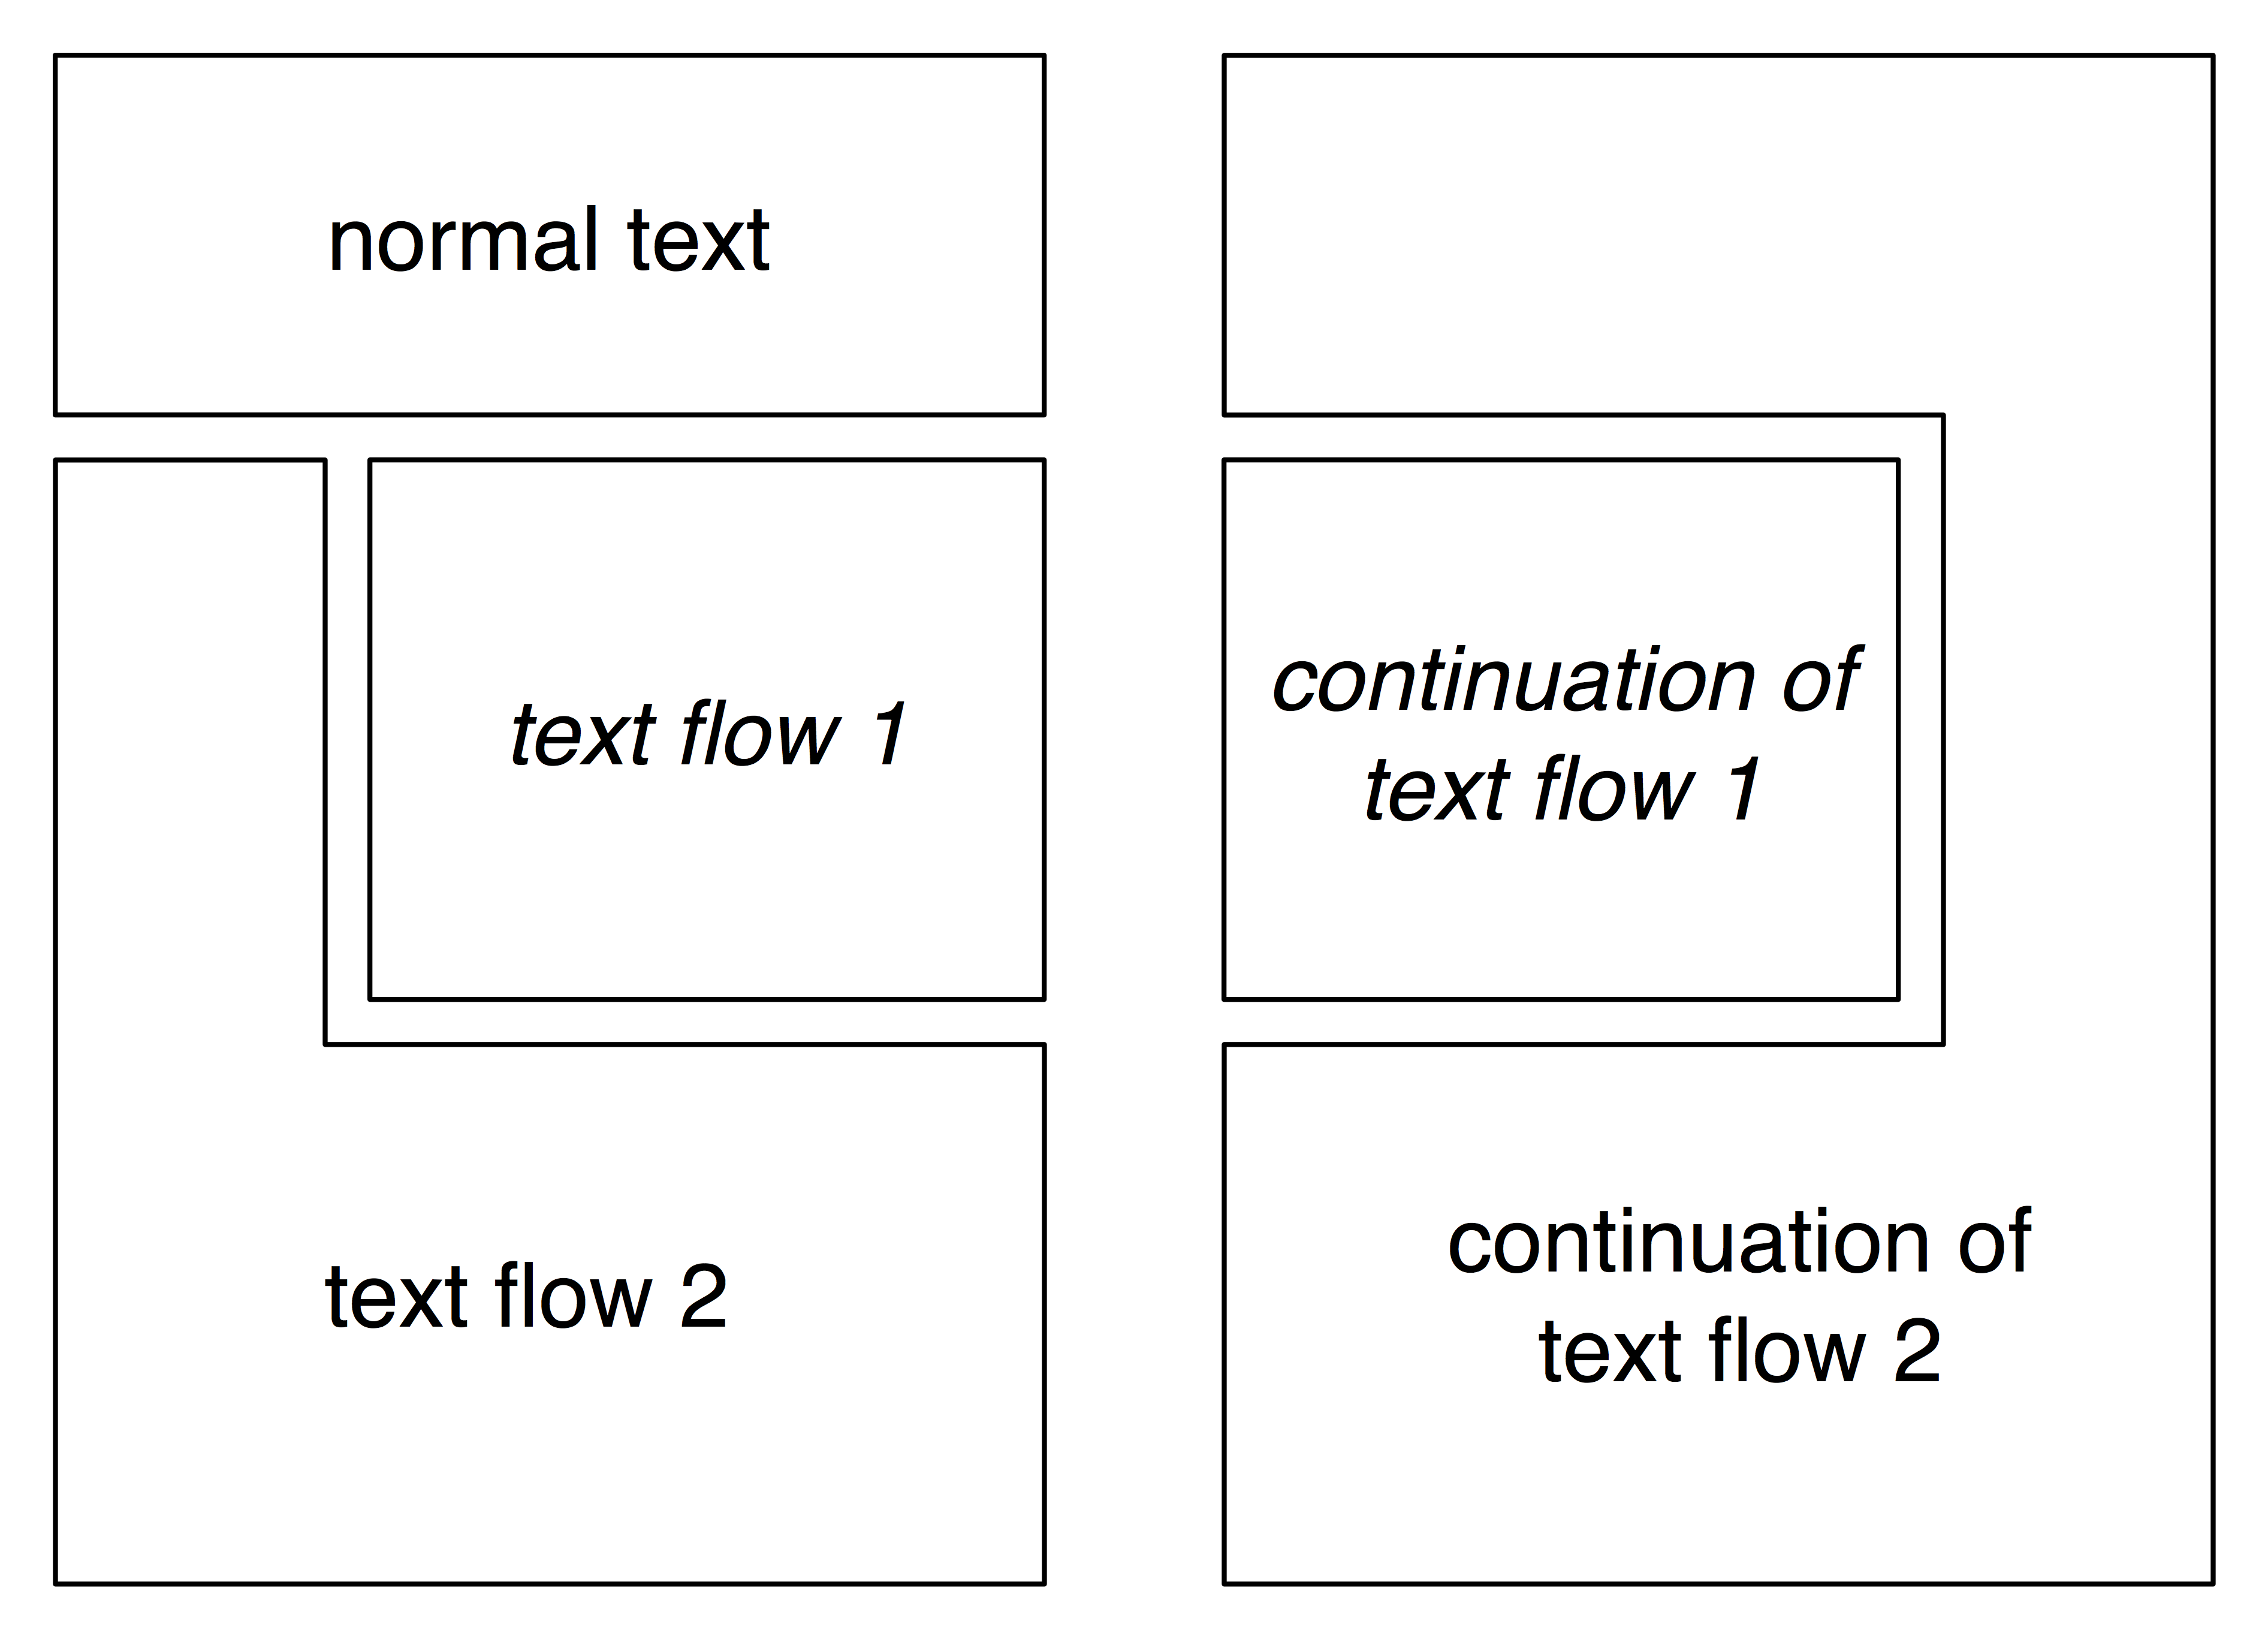
\includegraphics[width=12cm]{two_textflows.png}

\begin{typeLatin}
\bold{<pb>} \\
normal text \\
\bold{<tf 1 it>} \\
text flow 1 \\
\bold{</tf>} \\
\bold{<tf 2>} \\
text flow 2 \\
\bold{</tf>} \\ \\
\bold{<pb>} \\
\bold{<tf 1 it>} \\
continuation of \\ 
text flow 1 \\
\bold{</tf>} \\
\bold{<tf 2>} \\
continuation of \\ 
text flow 2 \\
\bold{</tf>} \\
\end{typeLatin}
\end{example}

\section{Anchored Comments}

\begin{mainrule}
Anchored comments are marked by §<ac> </ac>§. The anchor is treated like a footnote symbol, i.e. it is marked by §<n>§ in the first text flow and it is typed inside the §<ac>§ tag in the second text flow. In the second text flow, type the text after the anchor up to the~§]§ between §<ac>§ and §</ac>§.
\end{mainrule}

\begin{clarification}
The anchor symbol in the first text flow may have an additional §¶§, e.g. §¶ a§ in the first text flow and §a§ in the second text flow. The anchors in the two text flows may not be on the same page.
\end{clarification}

\begin{sampleImage}{anchorednote_conim_395}

\begin{typeLatin}
\bold{<tf 1 it>} \\
\bold{<h>_}CAPVT X.\bold{_</h>} \\
\bold{<p>}D \bold{<n} a\bold{>} E oppo$itis autem, quot modis opponi $oleant, de-\\
inceps dicend\~u e$$e videtur. \bold{<n} ¶ b\bold{>} Oppo$ita nanq; mo\\
dis quatuor opponi dicuntur: aut vt ea quæ $unt ad\\
aliquid: aut vt contraria, aut vt habitus, & priua-\\
tio, aut vt affirmatio atq; negatio. Atq; vt in $umma dicam du-\\
plum, & dimidium, vt ea, quæ $unt ad aliquid: bonum & mal\~u,\\
vti contraria: cæcitas atque vi$us, vt habitus, & priuatio: $edere, \\
\someText\bold{</p>} \\
\someText \\
\bold{</tf>} \\
\bold{<tf 2>} \\
\bold{<h>}COMMENTARIVS.\bold{</h>} \\
\bold{<p>}\bold{<ac} a\bold{> _}De oppo$itis autem.\bold{_}]\bold{</ac>} \\
Hæc e$t tertia, & vlti-\\
ma pars huius tractatus\\
in qua nonnulla declarã\\
tur, quorum mentio in\\
tradendis prædicamen-\\
tis facta e$t, & plenior\~e\\
de$iderabant explicat\~u;\\
hæc $unt contraria, qu\li{ae} \\
\someText\bold{</p>} \\
\someText \\
\bold{</tf>} \\
\end{typeLatin}
\end{sampleImage}

%\someText \\
%\bold{<n} ¶ c\bold{>} Sunt autem habitus quidem, & di$po$itiones: di$po$itiones ve \\
%\someText \\ 
%\bold{<tf 2>} \\
%\someText \\
%\bold{<p><ac} c\bold{> _}Sunt autem habitus.\bold{_}]\bold{</ac>} Communis etc. \\
%\someText \\

\begin{note}
The anchored comment itself is typed after §</ac>§ tag.
\end{note}

\end{document}
